\documentclass[11pt,letterpaper]{article}
\usepackage{amsmath}
\usepackage{amsfonts}
\usepackage{amssymb}
\usepackage{fullpage}
\usepackage{graphicx}
\usepackage[normalem]{ulem}
\usepackage{url}

\begin{document}

\begin{center}
\huge
\textsc{Smart Refrigerator Design Project}\\
\Large
\textsc{Progress Report V} \\
\vspace{.20cm}
\hrule
\vspace{.40cm}
\normalsize
Steven Strapp, Ben Reeves, Dustin Stroup \\
\today \\
\vspace{1cm}
\end{center}

\section{Updated Milestone Chart}
\begin{table}[h!]
\begin{center}
\begin{tabular}{| p{3.5 cm} | p{2 cm} | p{2 cm}| p{2 cm} | p{6 cm} | }
\hline
\textbf{Milestone} & \textbf{Scheduled Date} & \textbf{Assigned} & \textbf{Modified Date} & \textbf{Comments} \\
\hline
BeagleBoard \newline procured & February 10, 2012 & SS & NA & Complete \\
\hline
Angstrom operating system running on board & February 24, 2012 & DS & NA & Complete \\
\hline
Peripherals properly interfacing with \newline board & March 02, \newline 2012 & DS & March 30, \newline 2012 & Complete aside from temperature sensor. Was not considered in \newline original timeline. \\
\hline
Basic mobile UI, \newline suitable for \newline debugging & March 09, \newline 2012 & BR & NA & Complete \\
\hline
Basic base station UI, suitable for \newline debugging & March 09, \newline 2012 &SS & NA & Completed basic GUI functionality. Incorporating duplicate item \newline support and databases. \\
\hline
Database I/O \newline configured & March 16, \newline 2012 & DS &  March 23, \newline 2012 & MySQL databases configured, can be accessed with Python \newline application. \\
\hline
Testing and \newline integration of \newline temperature and \newline humidity sensor & March 16,  \newline 2012 &SS/DS & April 20, \newline 2012 & Partially complete. Tested using Arduino. Beagleboard GPIO \newline interface configured, needs testing. \\
\hline
Database and web server hosted by\newline Beagleboard & March 16, \newline 2012 & DS & NA & Complete \\
\hline
Beagleboard \newline touchscreen display procured & March 16, \newline 2012 & DS & NA & Complete \\
\hline

\end{tabular}
\end{center}
\end{table}

\begin{table}[h!]
\begin{center}
\begin{tabular}{| p{3.5 cm} | p{2 cm} | p{2 cm}| p{2 cm} | p{6 cm} | }
\hline
\textbf{Milestone} & \textbf{Scheduled Date} & \textbf{Assigned} & \textbf{Modified Date} & \textbf{Comments} \\
\hline
Mobile application integrated with web server & March 30, \newline 2012 &BR & April 20, \newline 2012 & Database integration still required.\\
\hline
User profiling and statistical analysis & March 30,\newline 2012 & SS & April 6, \newline 2012 & Complete\\
\hline 
Shopping lists, item modification, basic \newline settings & March 30, \newline2012 & SS & & Complete. Added context \newline menus and hidden ``administrator" panel. \\
\hline
Updated base station UI & April 6,\newline 2012 & SS & & Complete, awaiting review by team or outside testers.\\
\hline
Updated mobile application & April 6, \newline2012 & BR & April 20, \newline 2012& \\
\hline
Improved robustness of mobile interface& April 13,\newline 2012 & DS & & Purpose of this task has become unclear. May remove.\\
\hline
Integration testing \newline and system \newline verification & April 13, \newline2012 & BR & April 27, \newline2012& \\
\hline
Web interface \newline development & April 20, \newline 2012 & SS & & Complete. Does not look flashy but is effective and functional. \\
\hline
System testing and demo preparation & April 20, \newline2012 & SS & April 27, \newline2012& \\
\hline
\end{tabular}
\label {MilestoneTable}
\end{center}
\end{table}

\quad \newline \quad
\quad \newline \quad
\quad \newline \quad
\quad \newline \quad

\pagebreak[4]

\section{Current Milestones}
\begin{table}[h!]
\begin{center}
\begin{tabular}{| p{3.5 cm} | p{2 cm} | p{2 cm}| p{2 cm} | p{6 cm} | }
\hline
\textbf{Milestone} & \textbf{Scheduled Date} & \textbf{Assigned} & \textbf{Modified Date} & \textbf{Comments} \\
\hline
Mobile application integrated with web server & March 30, \newline 2012 &BR & April 20, \newline 2012 & Database integration still required.\\
\hline
Updated mobile application & April 6, \newline2012 & BR & April 20, \newline2012& \\
\hline
Testing and \newline integration of \newline temperature and \newline humidity sensor & March 16,  \newline 2012 &DS & April 20, \newline 2012 & Partially complete. Tested using Arduino. Beagleboard GPIO \newline interface configured, needs testing. \\
\hline
Web interface \newline development & April 20, \newline 2012 & SS & & Complete. Does not look flashy but is effective and functional. \\
\hline
\end{tabular}
\end{center}
\end{table}

\section{Next Milestones}
\begin{table}[h!]
\begin{center}
\begin{tabular}{| p{3.5 cm} | p{2 cm} | p{2 cm}| p{2 cm} | p{6 cm} | }
\hline
Mobile application integrated with web server & March 30, \newline 2012 &BR & April 20, \newline 2012 & Database integration still required.\\
\hline
Updated mobile application & April 6, \newline2012 & BR & April 20, \newline2012& \\
\hline
Testing and \newline integration of \newline temperature and \newline humidity sensor & March 16,  \newline 2012 & DS & April 20, \newline 2012 & Partially complete. Tested using Arduino. Beagleboard GPIO \newline interface configured, needs testing. \\
\hline
System testing and demo preparation & April 20, \newline2012 & SS & April 27, \newline2012& \\
\hline
\end{tabular}
\end{center}
\end{table}

\section{Status}
\begin{itemize}
\item Base station user interface and processing completed; awaiting possible aesthetic revisions following inclusion of the touch screen.
\item The web interface is complete. It was implemented using a simple HTML front end and PHP queries to MySQL database.
\item The mobile interface needs to be integrated with the MySQL databases. ORMLite can not interact with MySQL databases and research indicates Android can not interact with remote databases directly. This interface may require additional PHP back end on the server side.
\item SciPy packages have been installed and Python interface is functioning correctly again.
\item Temperature sensor needs to be debugged and included. Touchscreen drivers need to be updated; screen orientation has been corrected but touch functionality is not working.
\end{itemize}
\pagebreak
\section{Gantt Chart}
\begin{figure}[h!]
\begin{center}
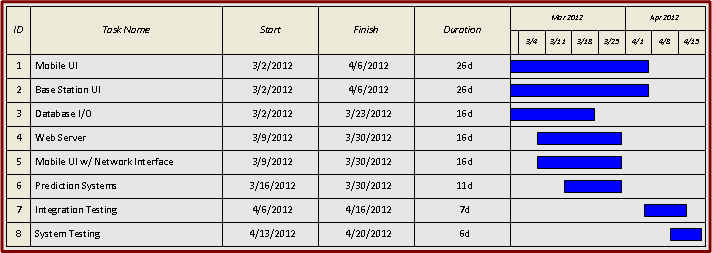
\includegraphics[scale=.6]{GanttChartI}
\end{center}
\end{figure}

\end{document}
